\section{Syntax trees and canonical derivations}

\begin{definition}
    A \emph{syntax tree} is a directed, ordered graph with no cycles, in which nodes are arranged from left to right, and for any pair of nodes, there is only one path connecting them.
\end{definition}
The key features of a syntax tree include:
\begin{itemize}
    \item It visually represents the derivation process.
    \item It has relationships such as parent-child, descendants, root node, and leaf (terminal) nodes.
    \item The degree of a node is determined by the number of its children.
    \item The root node represents the axiom $S$.
    \item The tree's frontier contains the generated phrase.
\end{itemize}
From a syntax tree, various subtrees can be defined by selecting a node $N$ as the new root.
\begin{example}
    The sentence $i+i*i$ can be represented in a syntax tree, following the rules for the sum and the product, as follows: 
    \begin{figure}[H]
        \centering
        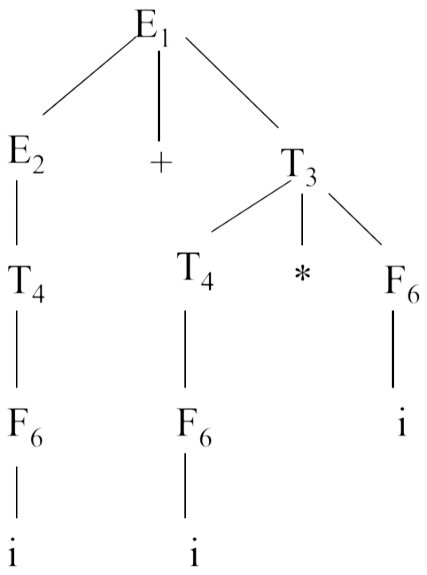
\includegraphics[width=0.25\linewidth]{images/syntree.png}
    \end{figure}
    It can also be written in a linear form: 
    \[[[[[i]_F]_T]_E+[[[i]_F]_T*[i]_F]_T]_E\]
\end{example}

We can have right (expands at each step the rightmost non-terminal) and left derivation (expands at each step the leftmost non-terminal). 
For a given syntax tree of a sentence, there exists a unique right derivation and a unique left derivation that correspond to that tree. 
Both right and left derivations are valuable for defining parsing algorithms.

The ambiguity of a grammar is determined by examining whether a given sentence has a unique syntax tree or not.

To construct a correct syntax tree, it's important to keep in mind the following:
\begin{itemize}
    \item Nonterminals for low-precedence operators are derived first.
    \item Nonterminals for high-precedence operators are derived later.
\end{itemize}
\begin{definition}
    A \emph{skeleton tree} is a syntax tree that preserves only the frontier and the structure. 

    A \emph{condensed skeleton tree} is a syntax tree where the internal nodes on a non-branching paths are merged. 
\end{definition}
\begin{example}
    The syntax tree from the previous example can be transformed into a skeleton tree:    \begin{figure}[H]
        \centering
        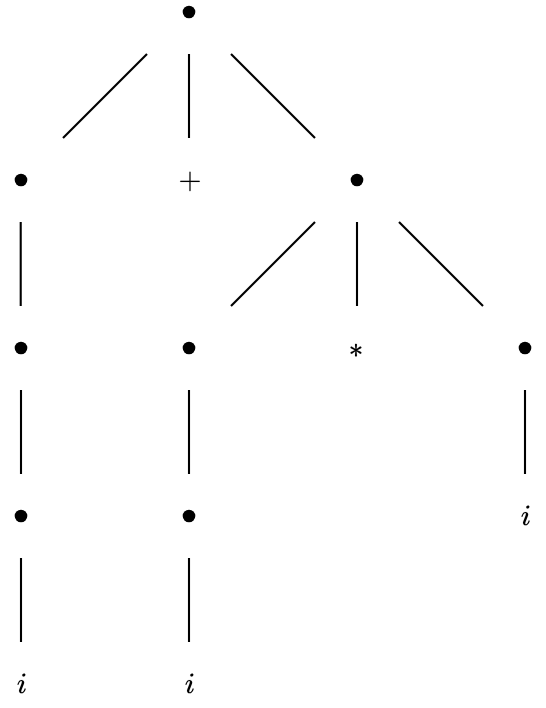
\includegraphics[width=0.2\linewidth]{images/syntree1.png}
    \end{figure}
    With the corresponding linear form:
    \[[[[[i]]]+[[[i]]*[i]]]\]
    It can also be transformed into a condensed skeleton tree:
    \begin{figure}[H]
        \centering
        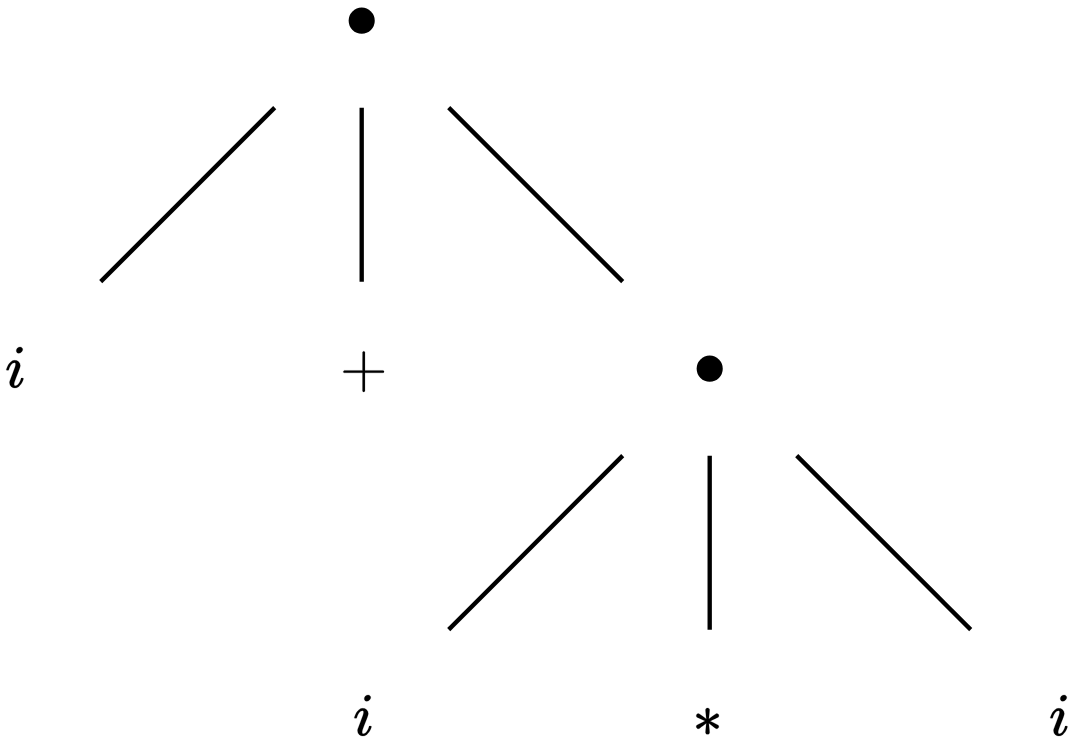
\includegraphics[width=0.2\linewidth]{images/syntree2.png}
    \end{figure}
    With the relative linear form:
    \[[[i]+[[i]*[i]]]\]
\end{example}